\documentclass[UTF8,a4paper]{ctexart}
\usepackage{graphicx}
\usepackage{geometry}
\geometry{a4paper,scale=0.9}
\usepackage{setspace}
\setstretch{1.6}

\begin{document}
\begin{sloppypar}
	
	\begin{center}
		\begin{fontsize}{80pt}{20pt}
			实验报告
		\end{fontsize}

		\bigskip
		\bigskip
		
		\begin{fontsize}{35pt}{20pt}
			\begin{flushright}
				———调试与性能分析、元编程及{\Huge Pytorch}的入门学习
			\end{flushright}
		\end{fontsize}
		
		\bigskip
		\bigskip
		\bigskip
		\bigskip
		\bigskip
		\bigskip
		\bigskip
		\bigskip
		\bigskip
		\bigskip
		\bigskip
		\bigskip
		\bigskip
		\bigskip
		\bigskip
		\bigskip
		\bigskip
		\bigskip
		\bigskip
		\bigskip
		\bigskip
		\bigskip
		
		\begin{fontsize}{25pt}{20pt}
			姓名:
			\underline{翟一航}
			
			\bigskip
			\bigskip
			\bigskip
			\bigskip
			
			学号:
			\underline{{\huge 23020011046}}
			
			\bigskip
			\bigskip
			\bigskip
			\bigskip
			
			班级:
			\underline{{\Huge 23}级软件工程五八班}
			
			
		\end{fontsize}
	\end{center}
	\section{实验要求}
	\subsection{学习代码的调试与性能分析}
	\subsection{简单学习元编程}
	\subsection{学习修改键位映射、VPN等大杂烩内容}
	\subsection{学习Pytorch的入门与应用}
	\section{实验内容}
	\subsection{学习代码的调试与性能分析}
	\subsubsection{代码调试与性能分析是软件开发中非常重要的两个方面,它们各自针对的问题和目的不同。}
	\subsubsection{代码调试是在软件开发过程中识别和修正代码中错误的行为。调试的目的是确保程序能够按照预期工作。调试过程通常包括以下几个步骤://1.错误重现:确定错误发生的条件和步骤,使得问题可以被稳定重现。//2.错误定位:通过阅读代码、设置断点、观察变量状态等方法找到错误的根源。//3.错误修正:修改代码中的错误,然后重新测试以验证问题是否已经被解决。//4.测试验证:确保修正错误的同时没有引入新的问题。}
	\subsubsection{调试工具和方法包括://1.打印语句:在代码中插入打印语句来输出变量值和程序状态。//2.集成调试器:大多数集成开发环境(IDE)都包含调试器,可以设置断点、单步执行、查看变量值等。//3.日志记录:通过日志记录程序的运行情况,帮助开发者了解程序的执行流程和状态。}
	\subsubsection{性能分析是指对软件程序运行时的性能进行测量和评估,目的是发现并解决性能瓶颈,提高程序的运行效率。性能分析通常关注以下几个方面://1.执行时间:测量程序或程序中某部分的执行时间。//2.资源使用:分析CPU、内存、磁盘I/O和网络的使用情况。//3.响应时间:对于交互式应用,关注的是用户操作到系统响应的时间。}
	
	\subsubsection{性能分析工具和方法包括://1.性能分析器:专门的工具,可以监控程序运行时的资源使用情况和函数调用情况。//2.基准测试:通过运行标准化的测试用例来评估性能。//3.代码剖析:对代码进行静态或动态分析,找出可能的性能问题。}
	\subsection{元编程的简单学习}
	\subsubsection{元编程是指编写可以操作其他程序代码的程序的过程。它可以使代码更加灵活、可重用和动态。元编程的应用非常广泛,包括构建系统、依赖管理、测试和持续集成系统等领域。}
	1.构建系统:构建系统是自动化构建过程的工具或系统,它负责将源代码转换为可执行程序。它可以包括编译、链接、打包等步骤。
	
	元编程的作用:通过元编程,构建系统可以根据不同的需求动态生成构建规则。例如,可以使用脚本生成构建配置文件,或者在构建过程中自动生成代码。
	
	2.依赖管理:依赖管理是处理项目中各个组件或库之间关系的过程。它确保项目在构建时能够找到和使用所需的库和资源。
	
	元编程的作用:依赖管理工具可以使用元编程技术来自动化依赖关系的解析和处理。例如,通过动态分析代码,工具可以自动检测并下载缺少的依赖。
	
	3.测试:测试是验证软件功能是否符合预期的过程,包括单元测试、集成测试和系统测试等。
	
	元编程的作用:在测试中,元编程可以用来自动生成测试用例、模拟对象或动态创建测试环境。例如,可以通过元编程生成各种输入数据,测试不同的代码路径。
	
	4.持续集成系统:持续集成系统自动化了软件开发过程中的构建、测试和部署步骤。它确保代码在集成到主分支之前能够通过所有测试。
	
	元编程的作用:在CI系统中,元编程可以用来自动化和定制化构建和测试流程。例如,CI系统可以根据不同的代码变更动态生成构建和测试任务。
	\subsection{大杂烩的学习}
	\subsubsection{修改键位映射}
	修改键位映射是指更改键盘上各个按键的功能,使它们执行不同于默认的操作。这可以通过操作系统的设置、专用的软件或工具来实现。例如,你可以将一个不常用的键重新映射为一个常用的快捷键,以提高使用效率或适应个人偏好。具体来说,修改键位映射可以让你定制键盘的行为,从而实现更加个性化的操作体验。
	\subsubsection{什么是守护进程}
	守护进程(Daemon)是指在后台运行的进程,它不依赖于用户的直接交互,而是执行系统或应用程序的服务任务。守护进程通常在系统启动时启动,并持续运行,直到系统关闭。它们可以处理各种任务,如网络服务、日志记录、系统监控等。守护进程的“守护”特性使它们能够在系统的后台安静地工作,确保服务的持续可用性。
	\subsubsection{备份}
	备份是指将重要数据或系统的副本存储在安全的位置,以防原始数据丢失或损坏。备份的目的是确保在数据丢失、硬件故障或其他灾难发生时,能够恢复数据或系统的正常功能。备份可以是完整的、增量的或差异的,依赖于备份的策略和需求。
	\subsubsection{Markdown}
	Markdown是一种轻量级的标记语言,用于格式化文本。它使用简单的标记符号来表示不同的文本格式,如标题、列表、粗体等。Markdown广泛用于编写文档、博客文章和README文件,因为它易于阅读和编辑,并且可以转换为HTML等格式。
	\subsubsection{Github}
	GitHub是一个基于Git的代码托管平台,提供版本控制和协作功能。它允许开发者存储代码、跟踪版本、管理项目以及与其他开发者协作。GitHub支持代码审查、问题跟踪、拉取请求等功能,促进团队开发和开源项目的管理。
	\subsection{pytorch的学习}
	\subsubsection{PyTorch是一个开源的机器学习库,由Facebook的人工智能研究团队开发,用于应用如计算机视觉和自然语言处理等领域的深度学习。PyTorch提供了两个主要功能://1.强大的张量计算与GPU加速支持。//2.动态计算图,可以提供完全的灵活性和速度。}
	PyTorch的关键特点:
	
	1.张量
	
	PyTorch中的基本数据结构是张量,它是一个多维数组,类似于NumPy的ndarray,但可以在GPU上使用以加速计算。
	
	2.动态计算图
	
	PyTorch使用动态计算图(也称为即时执行计算图),这意味着图的构建和修改可以在运行时进行,提供了很大的灵活性。这与静态计算图不同,后者需要先定义整个计算图然后再执行。
	
	3.自动微分
	
	PyTorch的autograd包提供了自动微分的功能。这对于执行深度学习中的反向传播算法特别有用。你可以定义一个计算图,并且autograd会自动为你计算梯度。
	
	4.灵活性和易用性
	
	PyTorch的设计哲学强调灵活性和易用性,使得研究人员可以快速实现想法,不需要花费大量时间编写底层代码。
	
	5.深度学习工具和库
	
	PyTorch拥有一个丰富的生态系统,包括各种工具和库,用于实现深度学习模型,如TorchVision用于图像处理,TorchText用于文本处理,TorchAudio用于音频处理等。
	
	6.社区支持
	
	PyTorch拥有一个活跃的社区,不断有新的研究和工具被集成进来。它的文档、教程和社区支持都非常丰富,这对于初学者和专业人士都非常有帮助。
	
	\subsection{课堂练习}
	\graphicspath{{figure/}}
	\subsubsection{使用 Linux 上的 journalctl 或 macOS 上的 log show 命令来获取最近一天中超级用户的登录信息及其所执行的指令。如果找不到相关信息,您可以执行一些无害的命令,例如 sudo ls 然后再次查看。}

	\bigskip
	\bigskip
	
	在虚拟机终端中输入journalctl | grep sudo,可以获取用户在最近的下载信息,按照时间数序排列。
	
	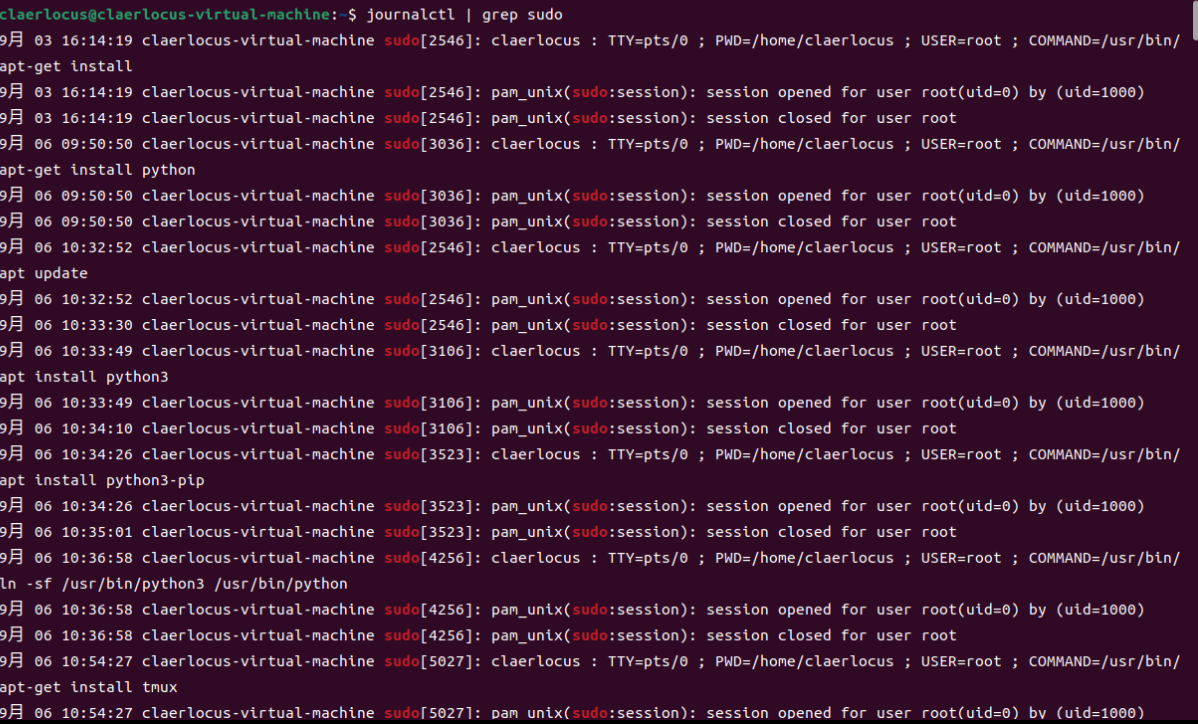
\includegraphics[width = 16cm]{1}
	
	然后输入sudo ls可以列出目录中的文件夹。
	
	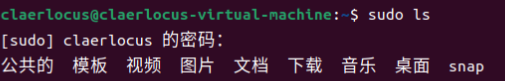
\includegraphics[width = 10cm]{2}
	
	\subsubsection{学习这份pdb 实践教程并熟悉相关的命令。更深入的信息您可以参考这份教程。}
	
	首先克隆下来该教程的Github仓库,然后进入下载下来的目录pbd-tutorial中
	
	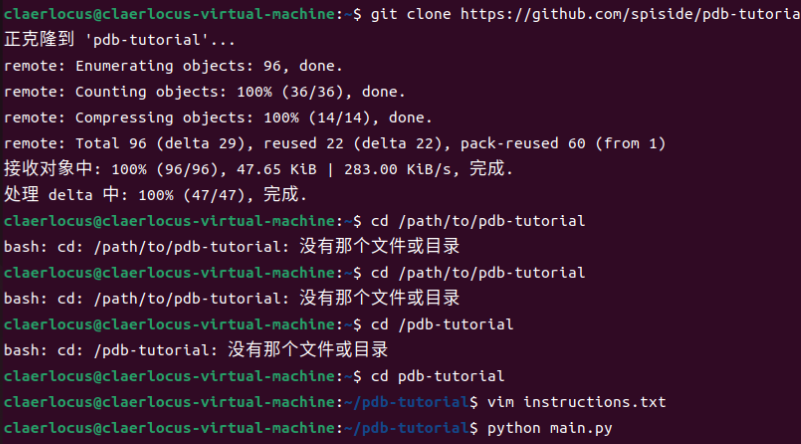
\includegraphics[width = 14cm]{3}

	然后使用vim查看其中的说明文件

	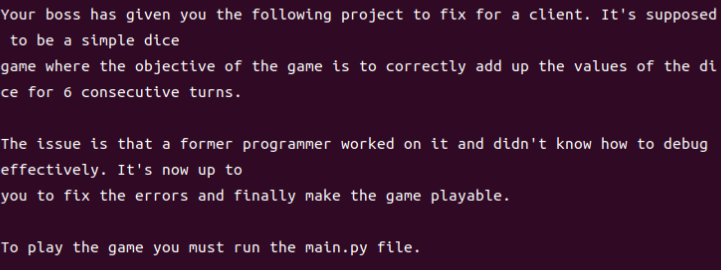
\includegraphics[width = 14cm]{4}
	
	运行main.py,得到如下结果:
	
	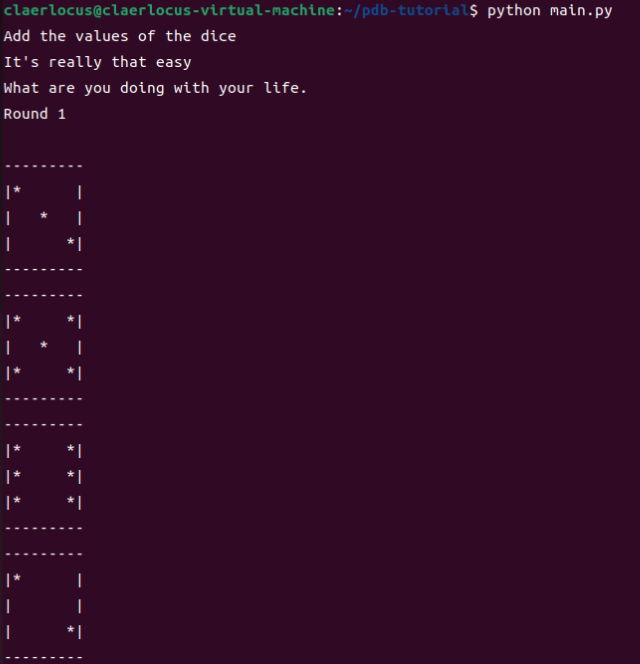
\includegraphics[width = 10cm]{6}
	
	发现程序运行发生错误,在程序中加入断点
	
	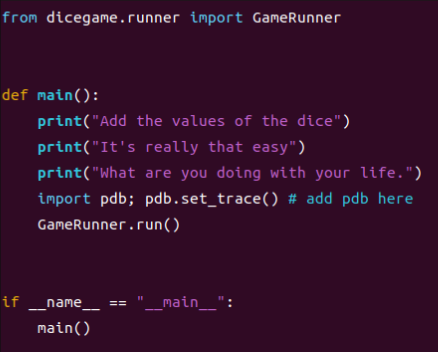
\includegraphics[width = 10cm]{5}
	
	然后进行程序的运行与调试,此处用python自带的pdb调试器对程序进行调试有几种不同的操作,分别为:l(ist) - 展示当前行附近的 11 行,或者是继续之前的展示、s(tep) - 执行当前行,会停在第一个可能停下的地方、n(ext) - 继续执行程序到当前函数的下一行或者是到它返回结果、b(reak) - 设置程序断点 (取决于提供的参数)、r(eturn) - 继续执行到当前函数返回结果。
	
	调试结果如下:
	
	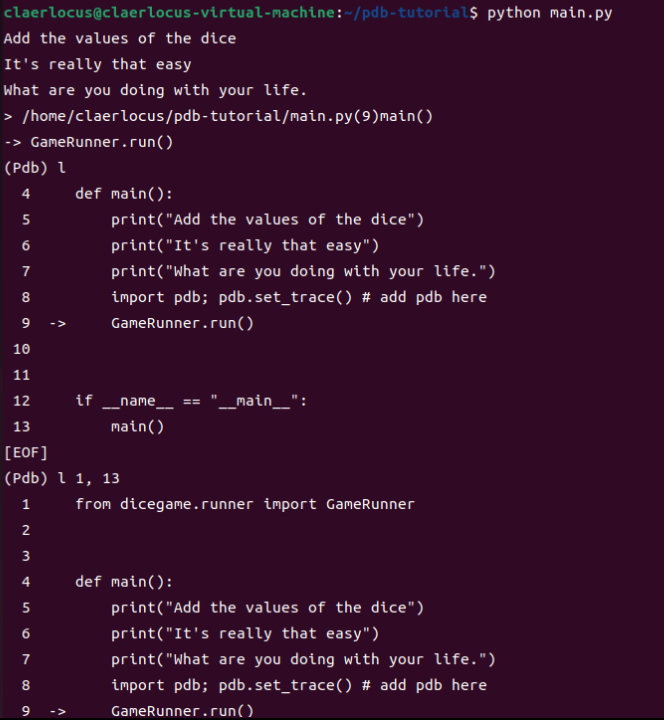
\includegraphics[width = 10cm]{7}
	
	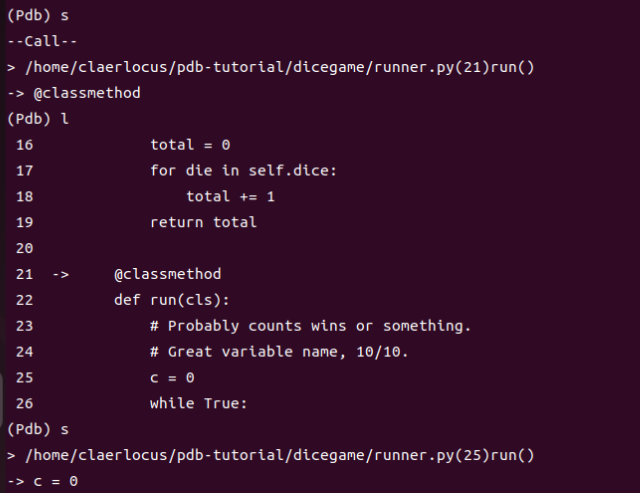
\includegraphics[width = 10cm]{8}
	
	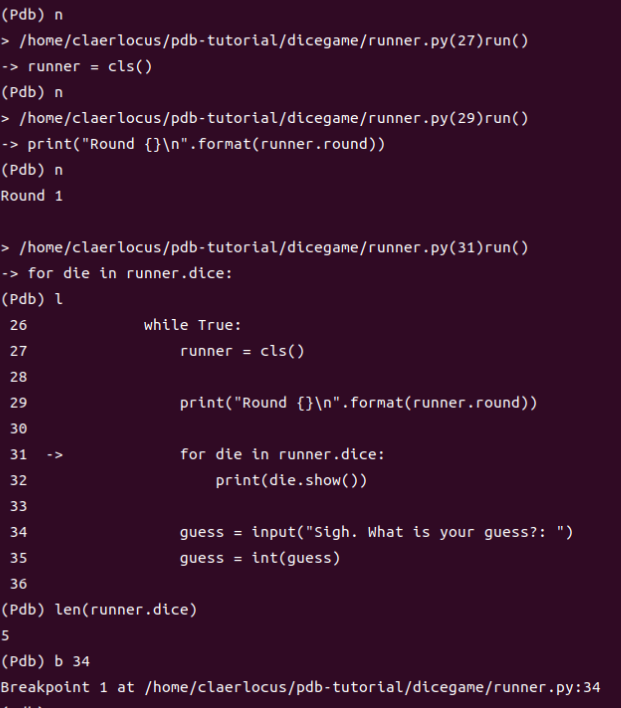
\includegraphics[width = 10cm]{9}
	
	\subsubsection{我们经常会遇到的情况是某个我们希望去监听的端口已经被其他进程占用了。让我们通过进程的 PID 查找相应的进程。首先执行 python -m http.server 4444 启动一个最简单的 web 服务器来监听 4444 端口。在另外一个终端中,执行 lsof | grep LISTEN 打印出所有监听端口的进程及相应的端口。找到对应的 PID 然后使用 kill <PID> 停止该进程。}
	首先在终端中输入命令python -m http.server 4444,启动一个最简单的 web 服务器来监听 4444 端口,如图:

	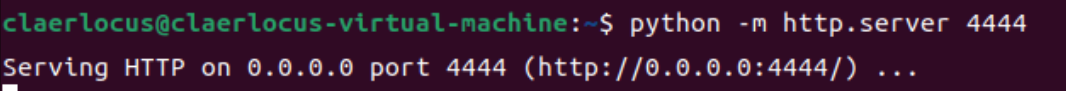
\includegraphics[width = 12cm]{10}

	然后再打开一个新的终端窗口,在其中执行命令lsof | grep LISTEN,打印出所有监听端口的进程及相应的端口,最后找到相应的pid,并使用kill命令将其终止。

	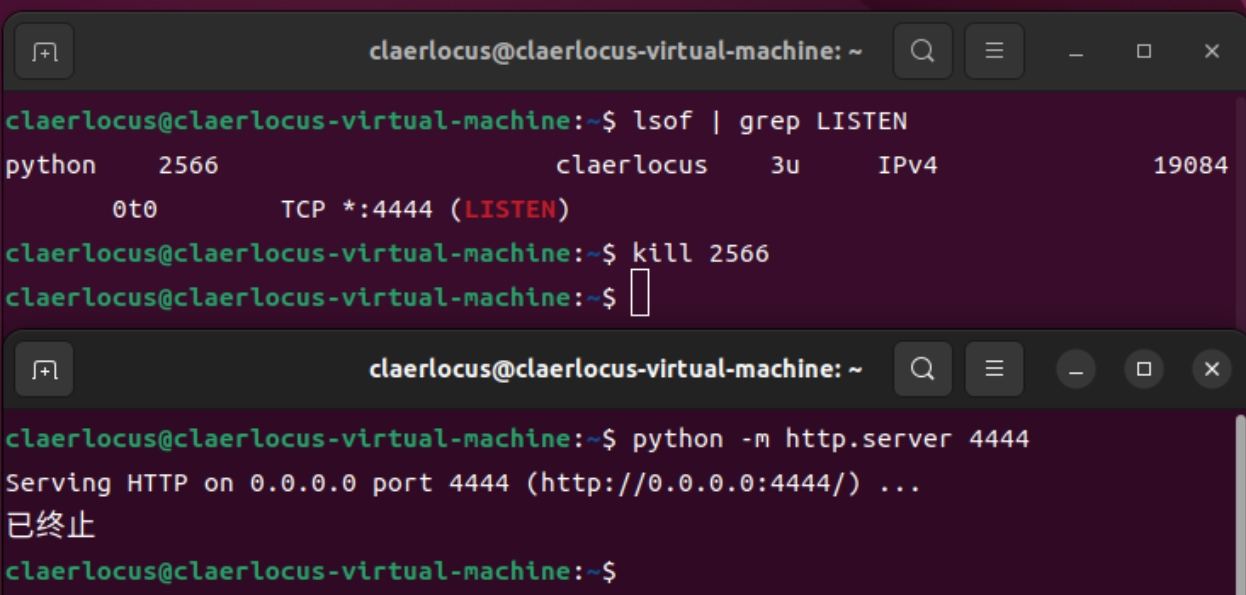
\includegraphics[width = 14cm]{11}
	
	\subsubsection{curl ipinfo.io 命令或执行 HTTP 请求并获取关于您 IP 的信息。打开 Wireshark 并抓取 curl 发起的请求和收到的回复报文。(提示:可以使用http进行过滤,只显示 HTTP 报文) 这里我使用的是curl www.baidu.com,请求百度的首页并过滤了除 HTTP 之外的其他报文}
	
	在终端中输入命令curl ipinfo.io,执行HTTP请求并获取IP信息,然后输入命令curl www.baidu.com来获取百度首页的信息,并对其进行抓包,去除图片等信息,只显示相应的HTML格式。

	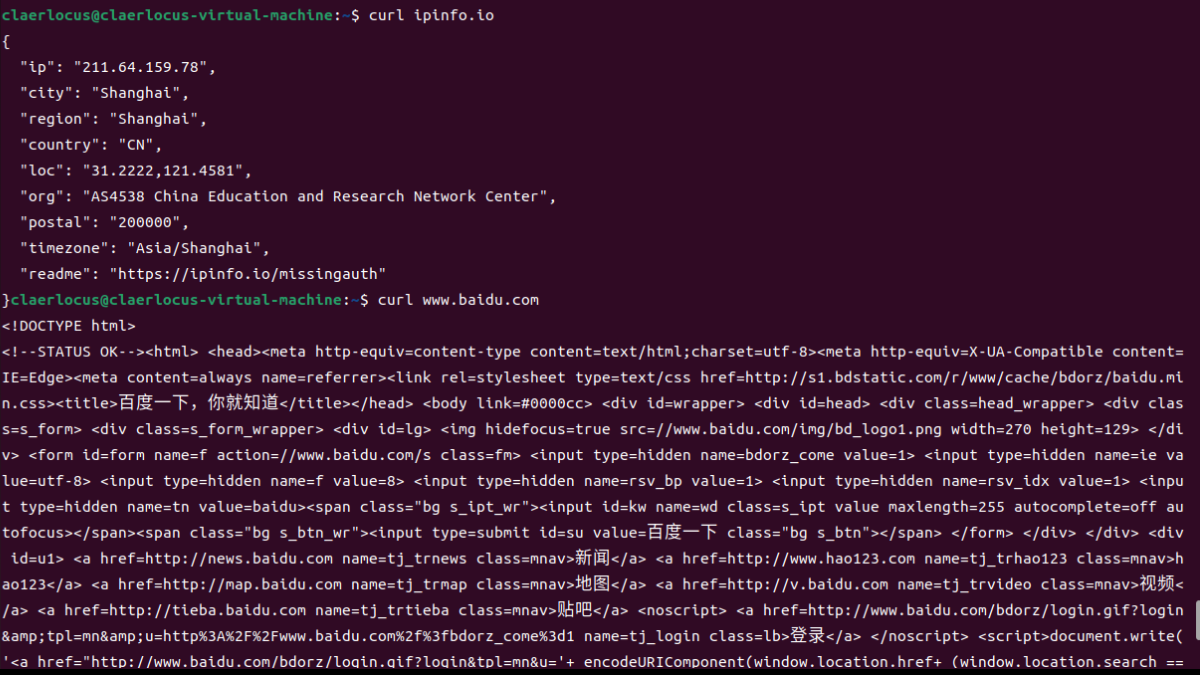
\includegraphics[width = 16cm]{12}

	
	\section{实验中遇到的问题与解决方法}
	\subsection{不知道如何启动pbd}

	在代码中插入 import pdb; pdb.set\_trace() 来设置一个断点。使用命令行参数-m来启动Python解释器,如:python -m pbd main.py。
	
	\subsection{在安装Anaconda时,由于未勾选配置选项,导致Anaconda与电脑上原本已有的python环境产生冲突而安装失败}
	
	重新进行Anaconda,并在安装时勾选相应的配置选项,且选择为all users安装该应用。

	\subsection{成功安装pytorch与cuda,再pycharm中进行pytorch运行环境的配置时,发现在Pycharm中进行python解释器的设置时,发现无法找到anaconda环境}
	
	在Anaconda下载的文件夹中找到aconda.bat文件,然后打开后通过local指令可以自动定位到揭示其配置所在位置,将其添加到pycharm的python解释器中即可。
	
	\section{实例练习}
	\subsection{使用打印调试法对python代码进行调试}
	首先在中孤单中写入一段简单的python代码,用来计算给定的两个参数的乘积,在程序中的特定位置加入print语句用来输出参数的值,便于进行程序的调试工作。

	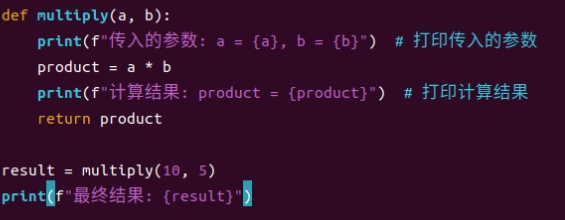
\includegraphics[width = 10cm]{13}
	
	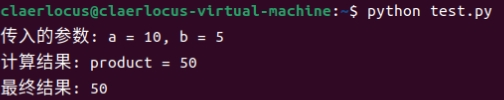
\includegraphics[width = 10cm]{14}
	
	\subsection{写一个简单加法程序,并使用pdb对程序进行调试}
	首先,创建一个名为debug\_example.py的文件,并在文件中写入如下代码,在想要开始调试的位置加入断点。

	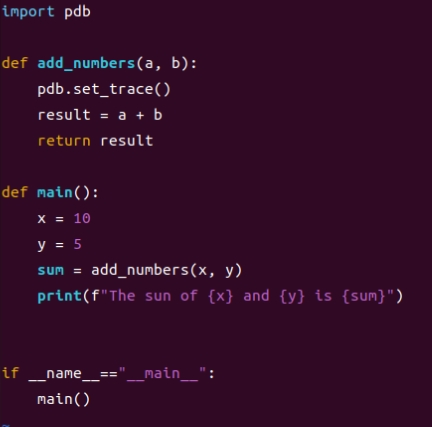
\includegraphics[width = 10cm]{15}
	
	然后运行该python程序,p 命令用于打印变量值,n 命令用于执行下一行代码。当你完成调试后,使用 quit 命令退出调试器。
	
	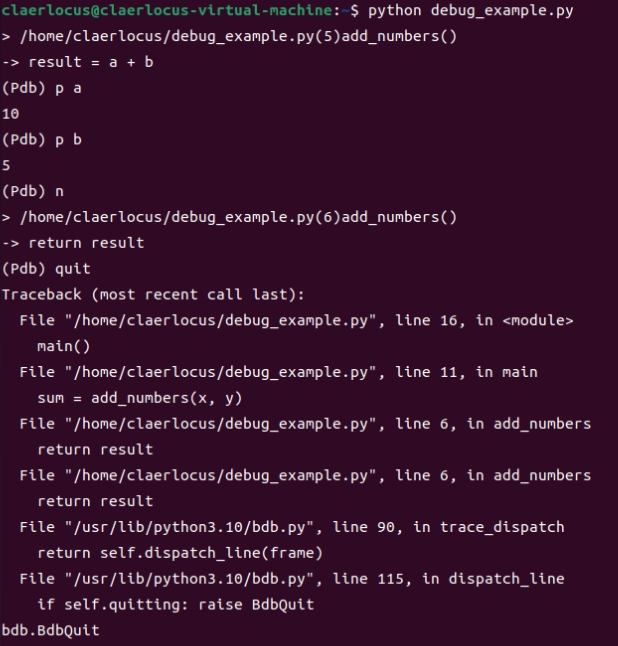
\includegraphics[width = 12cm]{16}

	\subsection{写一个简单的除法程序,并使用第三方日志系统对其进行调试}
	我们可以使用logging模块,它是Python标准库的一部分,功能强大且易于配置。在终端中创建一个.py类型的代码文件,并使用logging来记录调试信息。
	
	在程序中,我使用basicConfig函数配置了日志系统,包括日志级别和日志消息的格式,又定义了一个divide函数,在函数的关键点使用logging.debug()来记录调试信息,并在除数为零时使用logging.error()来记录错误信息。代码与运行结果如下图所示:
	
	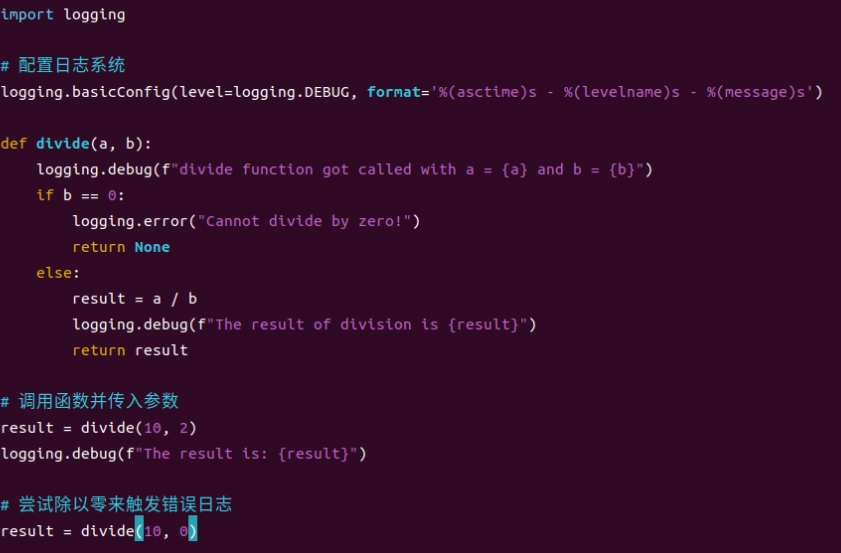
\includegraphics[width = 14cm]{17}
	
	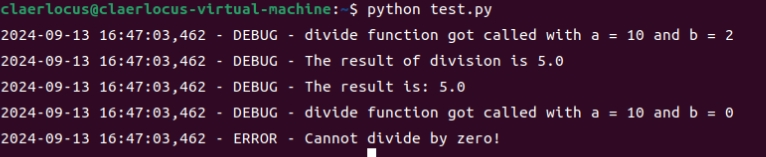
\includegraphics[width = 14cm]{18}
	
	\subsection{修改键位映射,将CapsLock与ctrl互换}
	首先现在终端中输入命令xmodmap -pke > keymap\_backup.txt,将现在的键位映射保存在文件中,方便在实验之后恢复键位。然后创建一个新的键位映射文件swap\_ctrl\_caps.xmodmap,并在其中写入交换Capslock与Ctrl的代码,然后使用命令xmodmap swap\_ctrl\_caps.xmodmap来创建新的键位。代码与运行结果如如下图所示:
	
	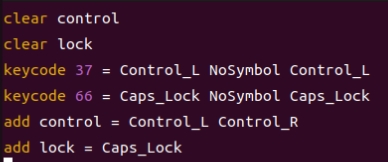
\includegraphics[width = 14cm]{19}
	
	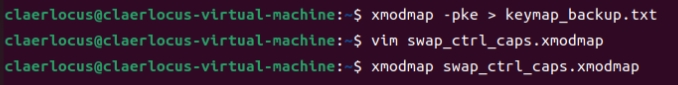
\includegraphics[width = 14cm]{20}
	
	\subsection{在终端中使用tar命令来进行文件的备份}
	首先在终端中创建一个文件example.txt,然后输入命令tar -czvf backup.tar.gz example.txt
	就可以将其保存到一个名为backup.tar.gz的压缩文件中
	
	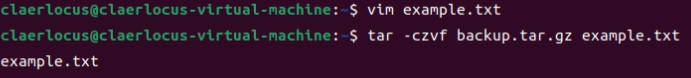
\includegraphics[width = 14cm]{21}
	
	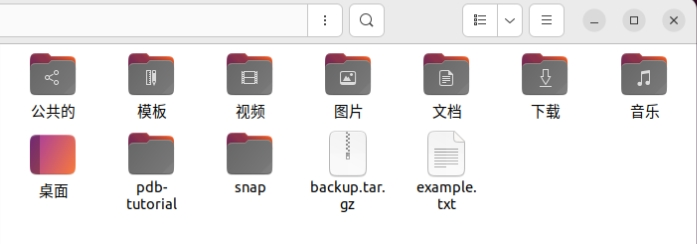
\includegraphics[width = 14cm]{22}
	
	\subsection{创建一个简单的应用程序接口(API)}
	先创建一个简单的TCP服务器示例,它监听一个端口,等待客户端连接,并接收并打印客户端发送的数据。另外为了确保给脚本执行权限,需要输入命令chmod +x simple\_tcp\_server.py,然后运行脚本。
	
	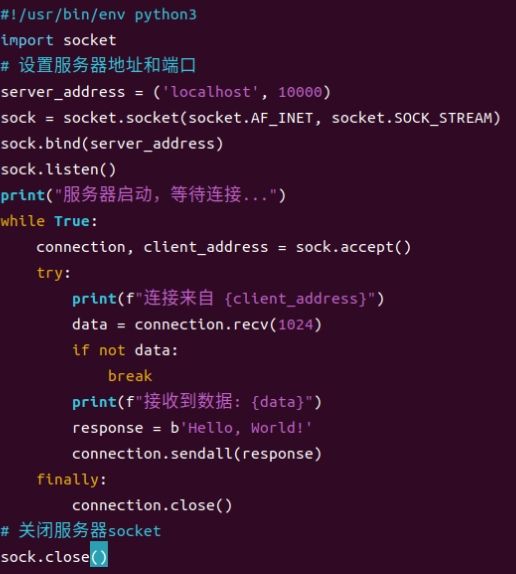
\includegraphics[width = 14cm]{23}
	
	在另一个终端窗口中,使用Python的socket库创建一个简单的TCP客户端,并连接到服务器,同样确保给脚本执行权限,然后运行脚本,可以发现客户端与服务器相连,并且打印出了客户端传递的内容。
	
	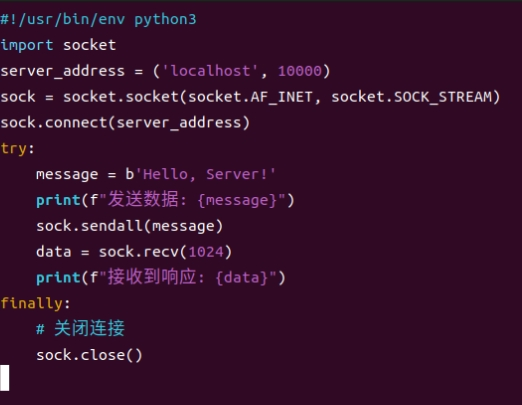
\includegraphics[width = 14cm]{24}
	
	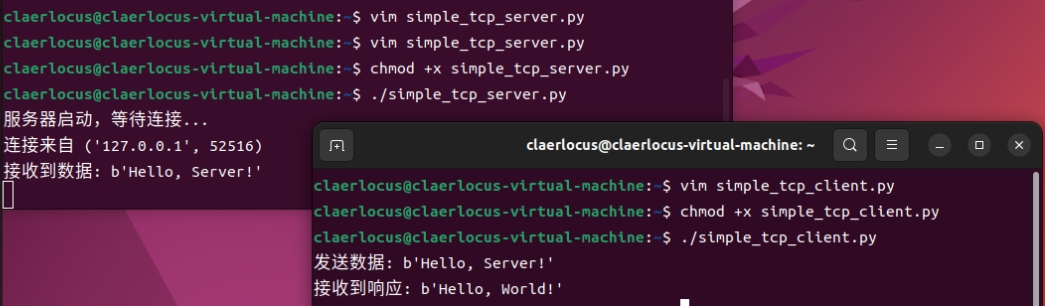
\includegraphics[width = 14cm]{25}
	
	\subsection{在markdown中设置标题}
	在文字之前加上\# 即可添加标题,随着\#数量的增加,总共有6级标题
	
	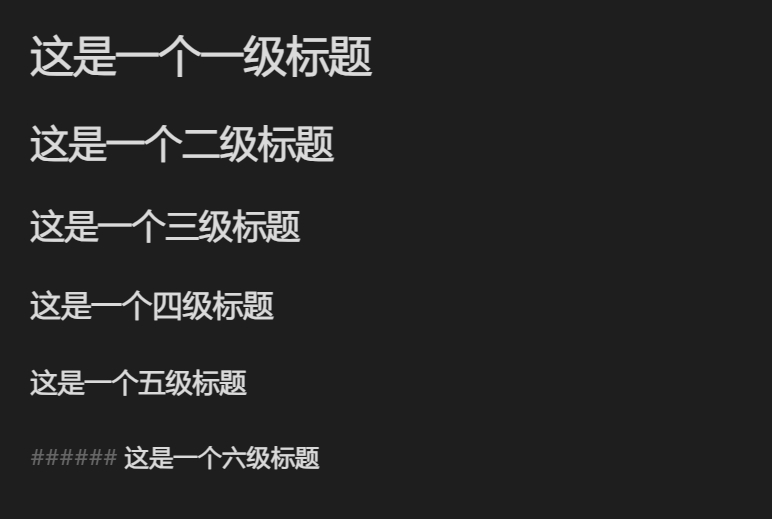
\includegraphics[width = 10cm]{26}
	
	\subsection{在markdown中使用*对字体进行处理}
	在文字内容两边加上*,会使输出的字体为斜体,在文字内容的两边加上**,会使文字内容加粗。
	
	
\includegraphics[width = 8cm]{27}
	
	
\includegraphics[width = 8cm]{28}
	
	\subsection{在markdown中输出矩阵}
	在markdown编辑器中输入如图代码,即可输出一个3阶矩阵。
	
	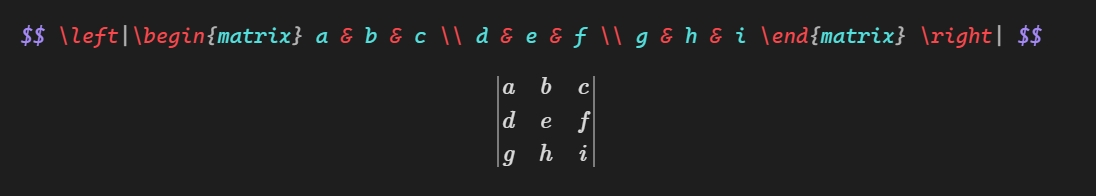
\includegraphics[width = 16cm]{29}
	
	\subsection{在markdown中输出任务括号}
	在markdown中可以输出任务括号,根据任务是否完成将括号勾选掉,实用方便。输入- \[\] 即可,要注意中括号的前后均有空格,效果如下图:
	
	
\includegraphics[width = 8cm]{30}
	
	\subsection{在markdown中输出代码与代码块}
	在要输入的代码前后用三个```符号将代码引用。
	
	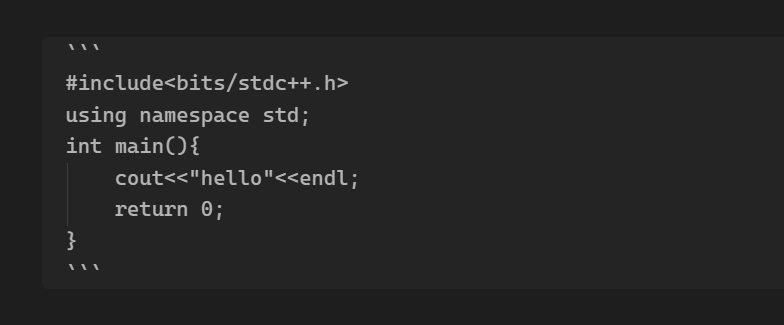
\includegraphics[width = 14cm]{31}
	
	\subsection{在markdown中插入超链接与图片}
	格式如下:[这是一个超链接/图片](超链接网址/图片地址)
	
	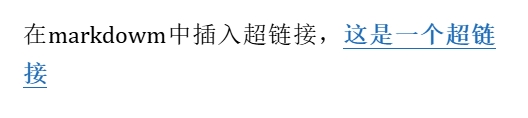
\includegraphics[width = 8cm]{32}
	
	\subsection{简易的神经网络}
	利用pytorch写一个简单的神经网络,程序与运行结果如下:
	
	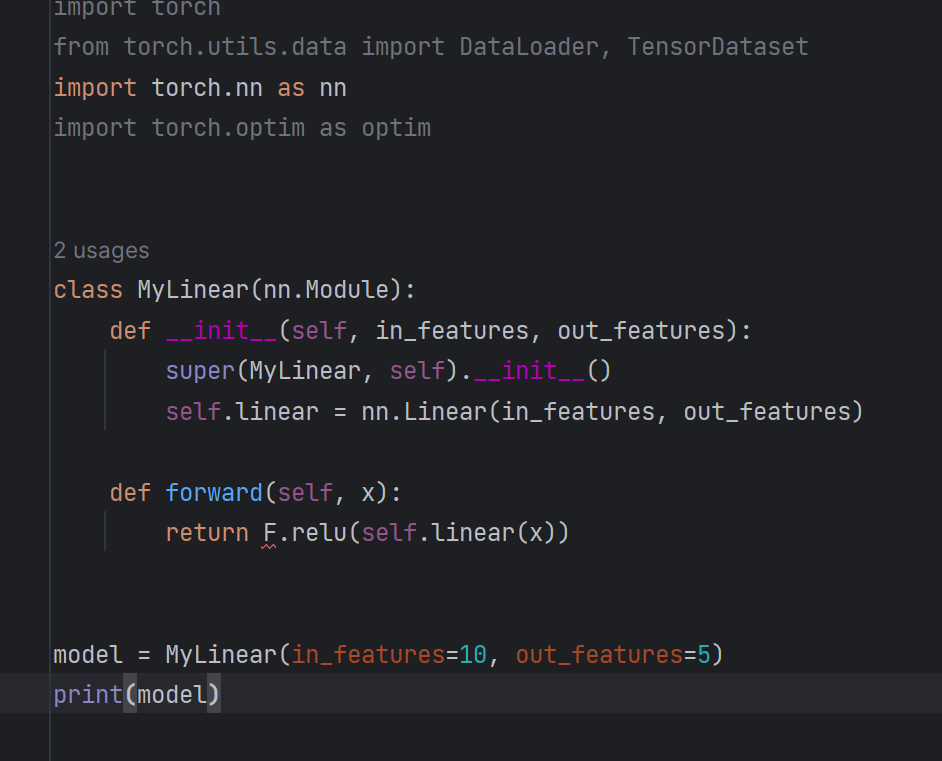
\includegraphics[width = 14cm]{33}
	
	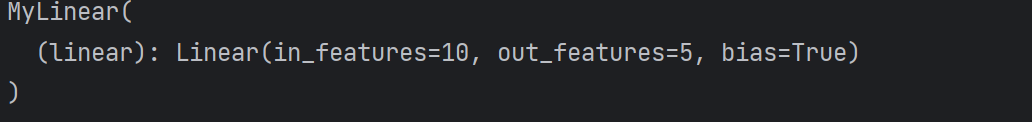
\includegraphics[width = 14cm]{34}
	
	\subsection{图像识别}
	使用PyTorch实现一个简单的卷积神经网络来识别MNIST手写数字。
	
	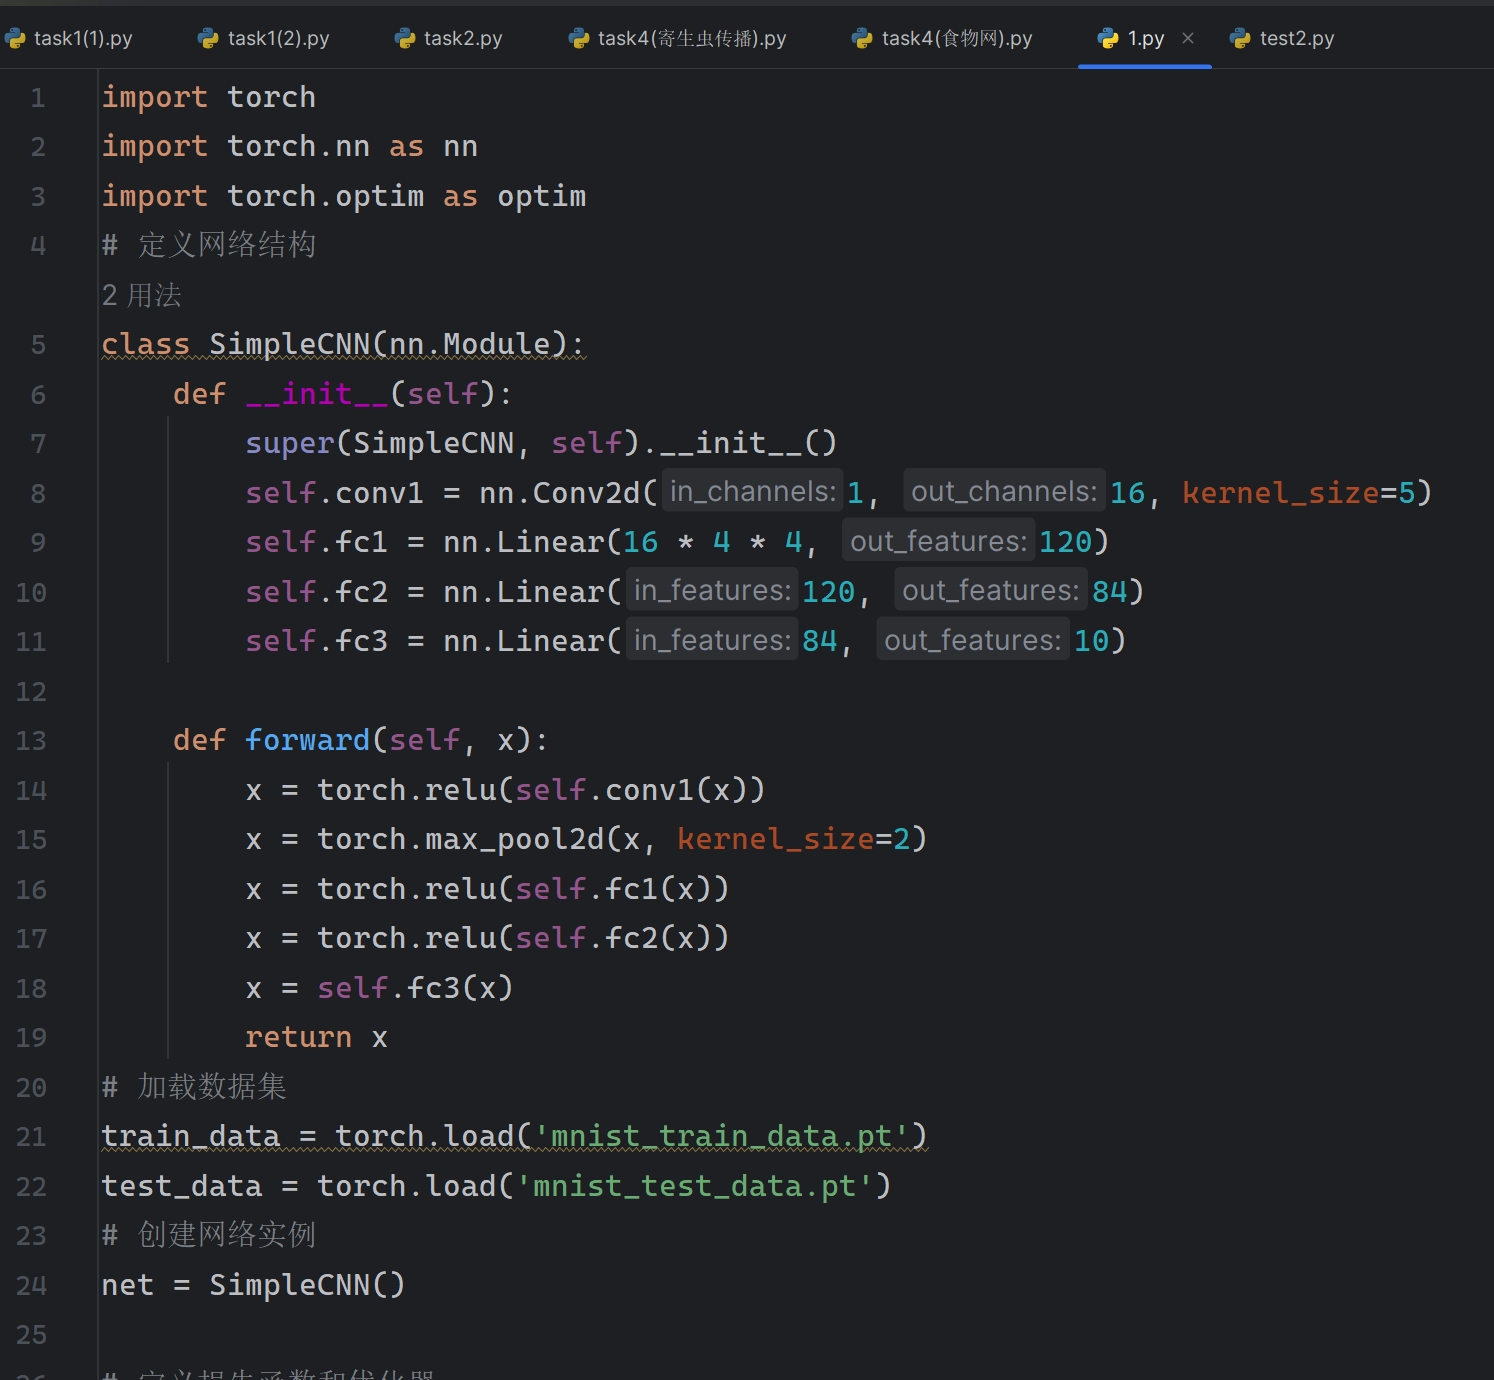
\includegraphics[width = 14cm]{35}
	
	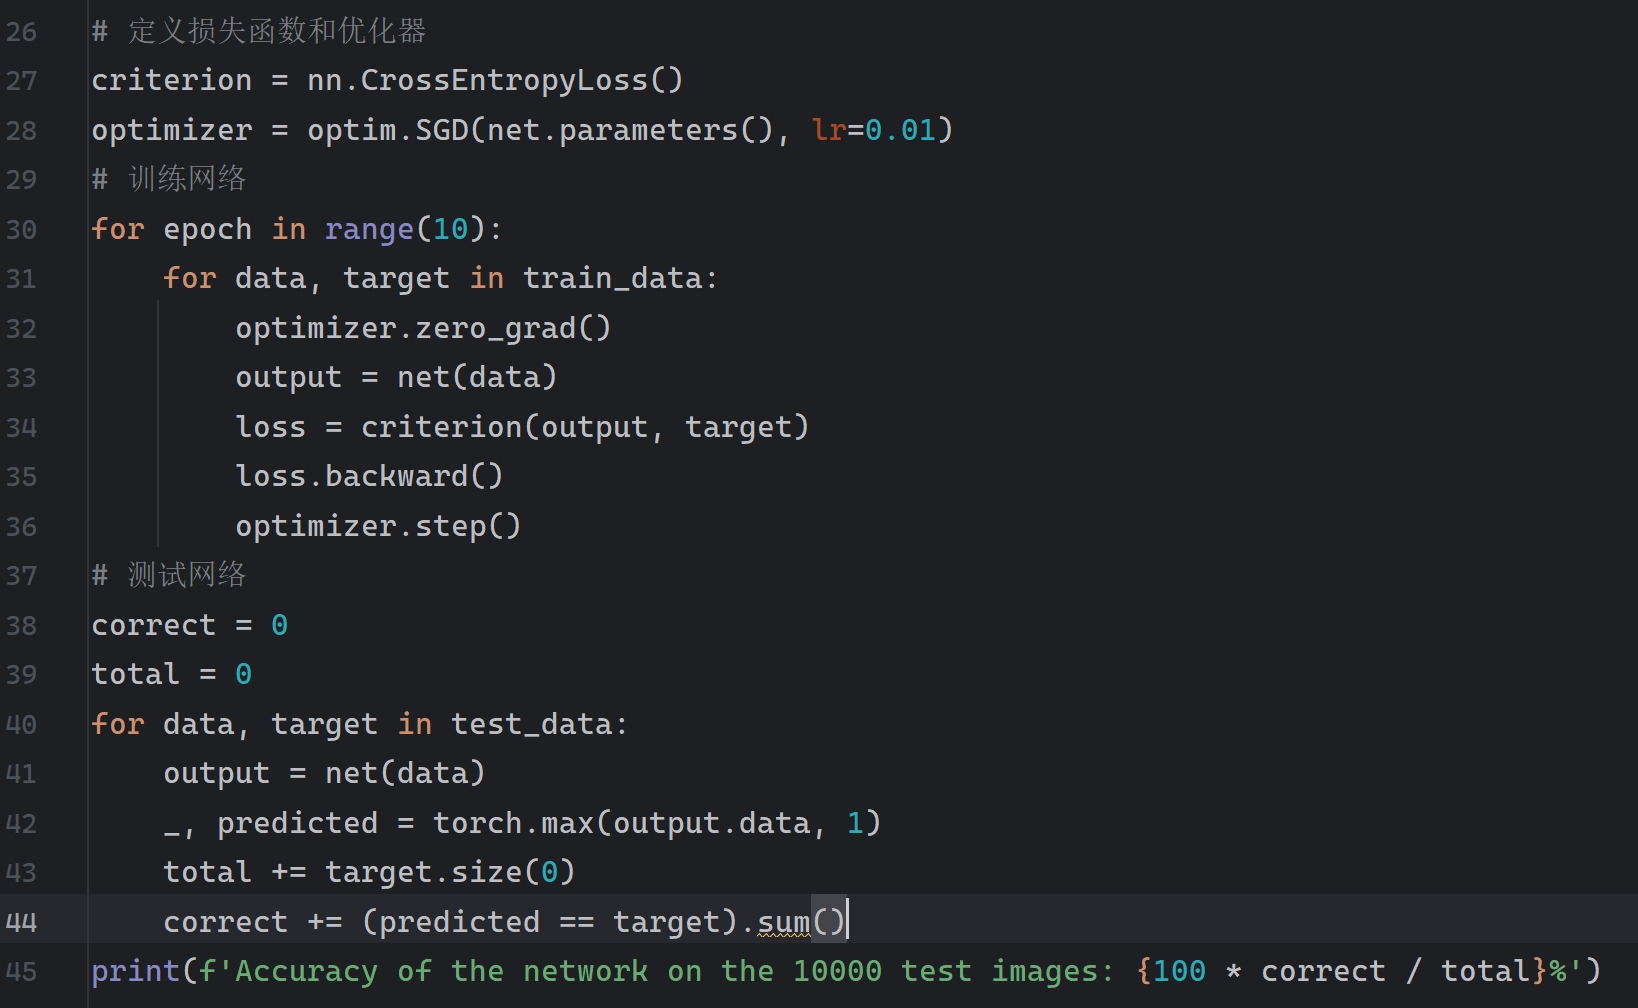
\includegraphics[width = 14cm]{36}
	
	在每个epoch结束时,代码将打印出当前epoch的编号和在该epoch结束时计算的损失值。
	
	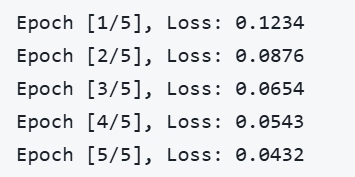
\includegraphics[width = 14cm]{36.1}
	
	在所有epoch训练完成后,代码将进入评估模式,计算模型在训练数据集上的准确率。
	
	
\includegraphics[width = 14cm]{36.2}
	
	\subsection{自然语言处理}
	使用PyTorch实现一个简单的循环神经网络来生成文本。
	 
	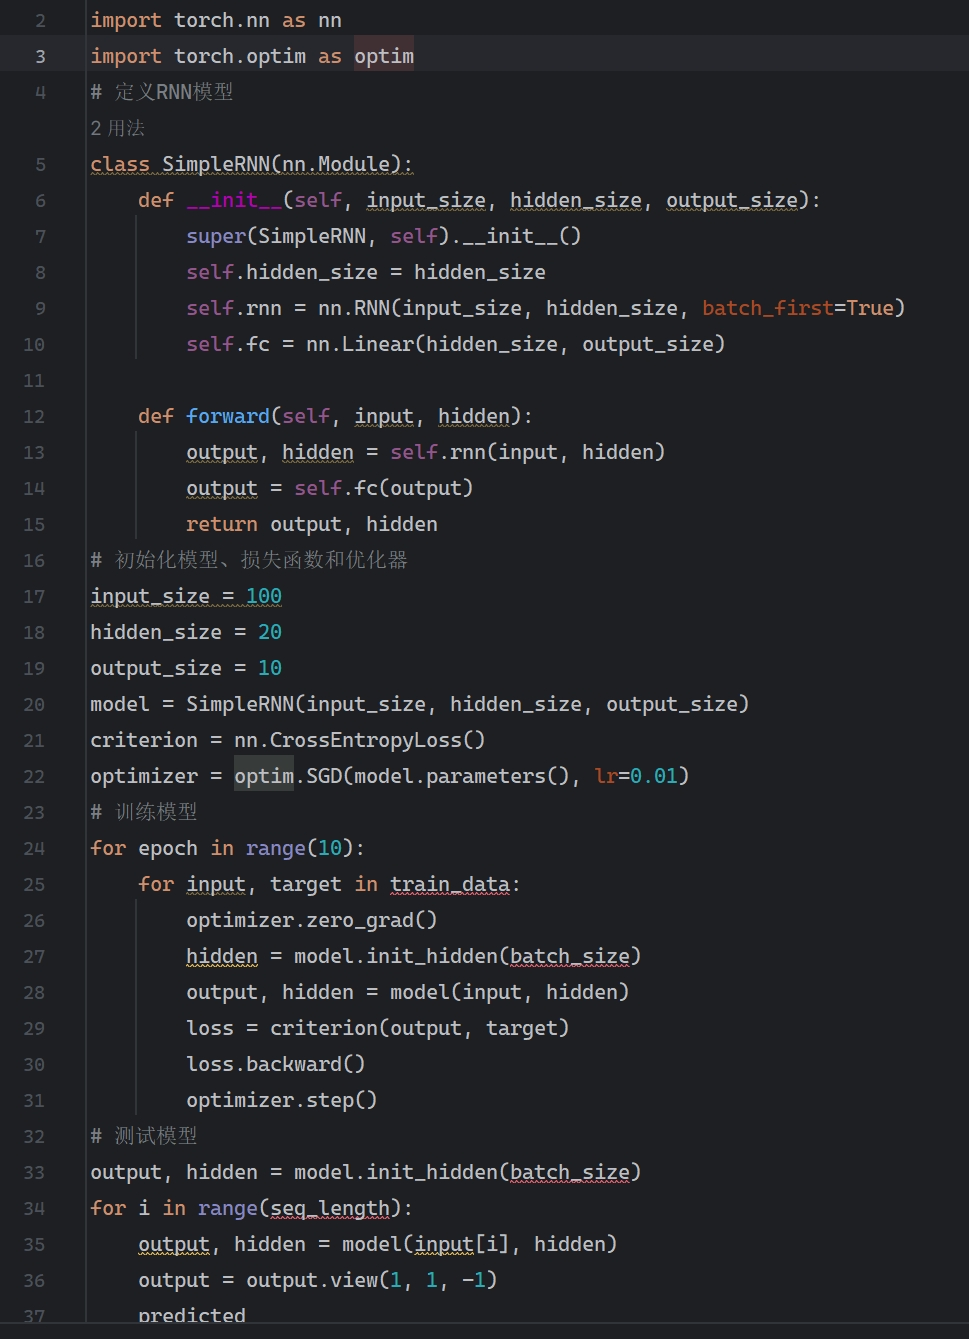
\includegraphics[width = 16cm]{37}
	
	在训练阶段,模型将会输出每个训练步骤的损失值,在生成文本阶段,generate 函数将使用模型来预测下一个字符,直到达到最大长度。
	
	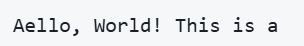
\includegraphics[width = 10cm]{37.1}
	
	\subsection{张量的基本操作}
	在这个实例中,我创建了一个PyTorch张量。张量是一个多维数组,可以在GPU上使用以加速计算,使pytorch中常见的量。初始化了一个包含两个浮点数和一个整数的列表,因为张量通常是同质的,所以会自动将整数转换为浮点数。然后打印出张量的内容、数据类型、形状等基本信息。
	
	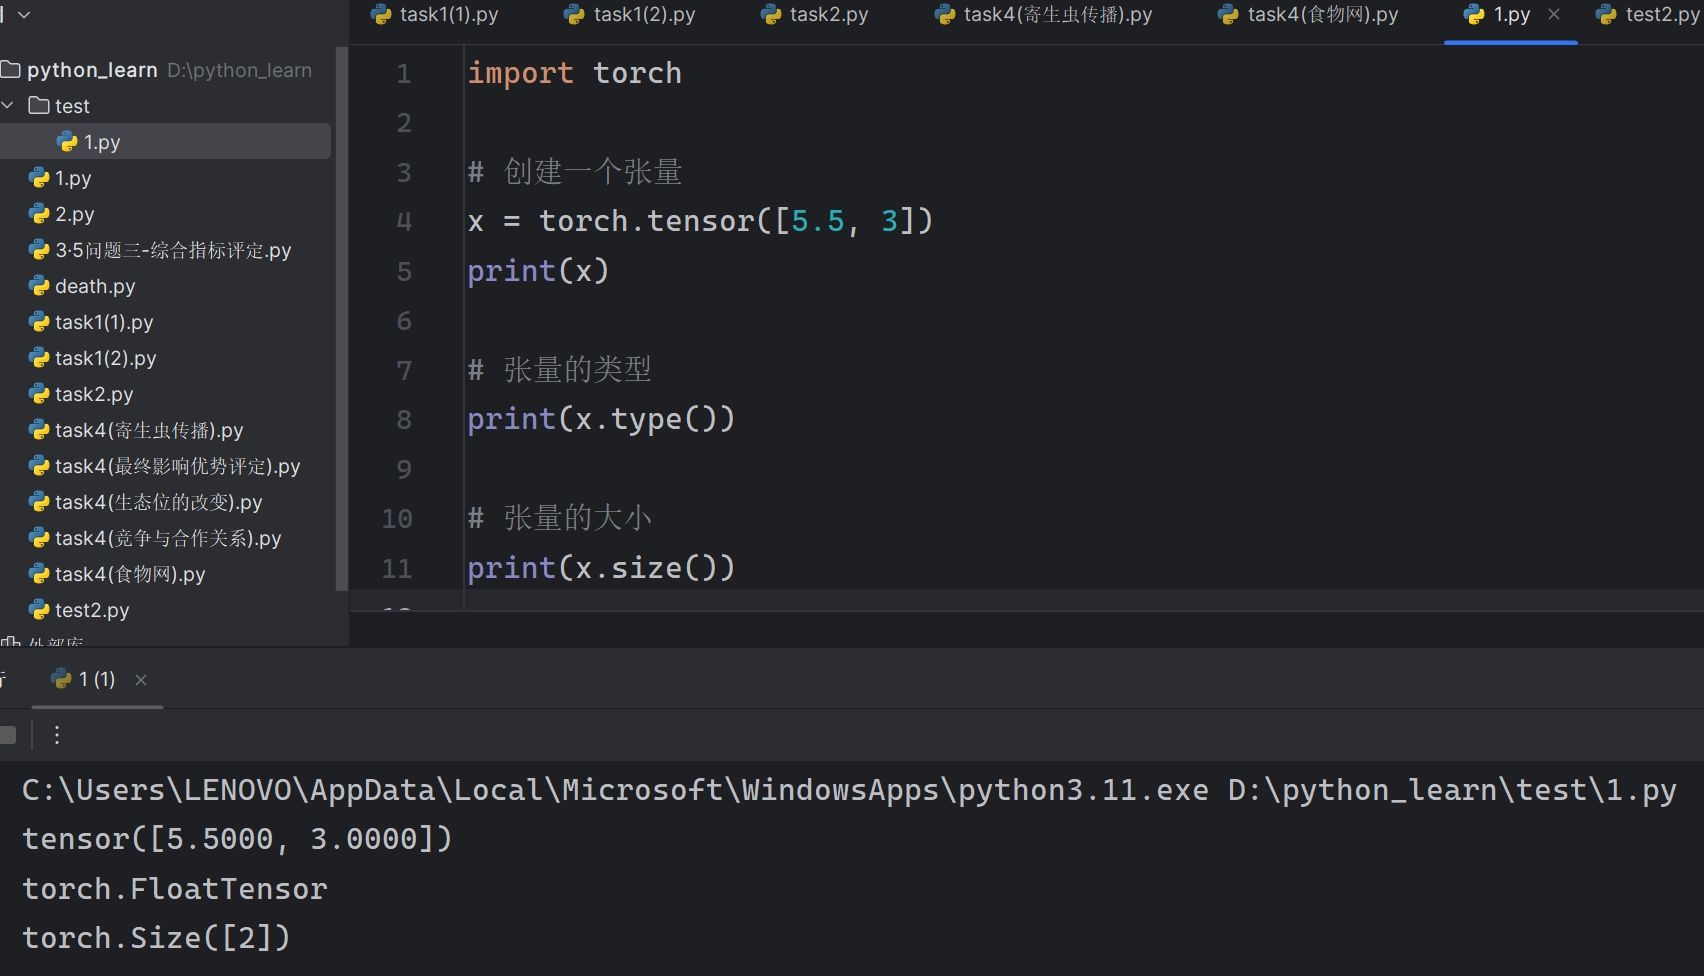
\includegraphics[width = 12cm]{38}
	
	\subsection{张量的运算}
	在这个实例中,我对两个张量x、y进行了简单的张量加法运算,得到了一个新的张量z,并将z输出。接着又对x和y进行点乘运算四年,并将结果输出。
	
	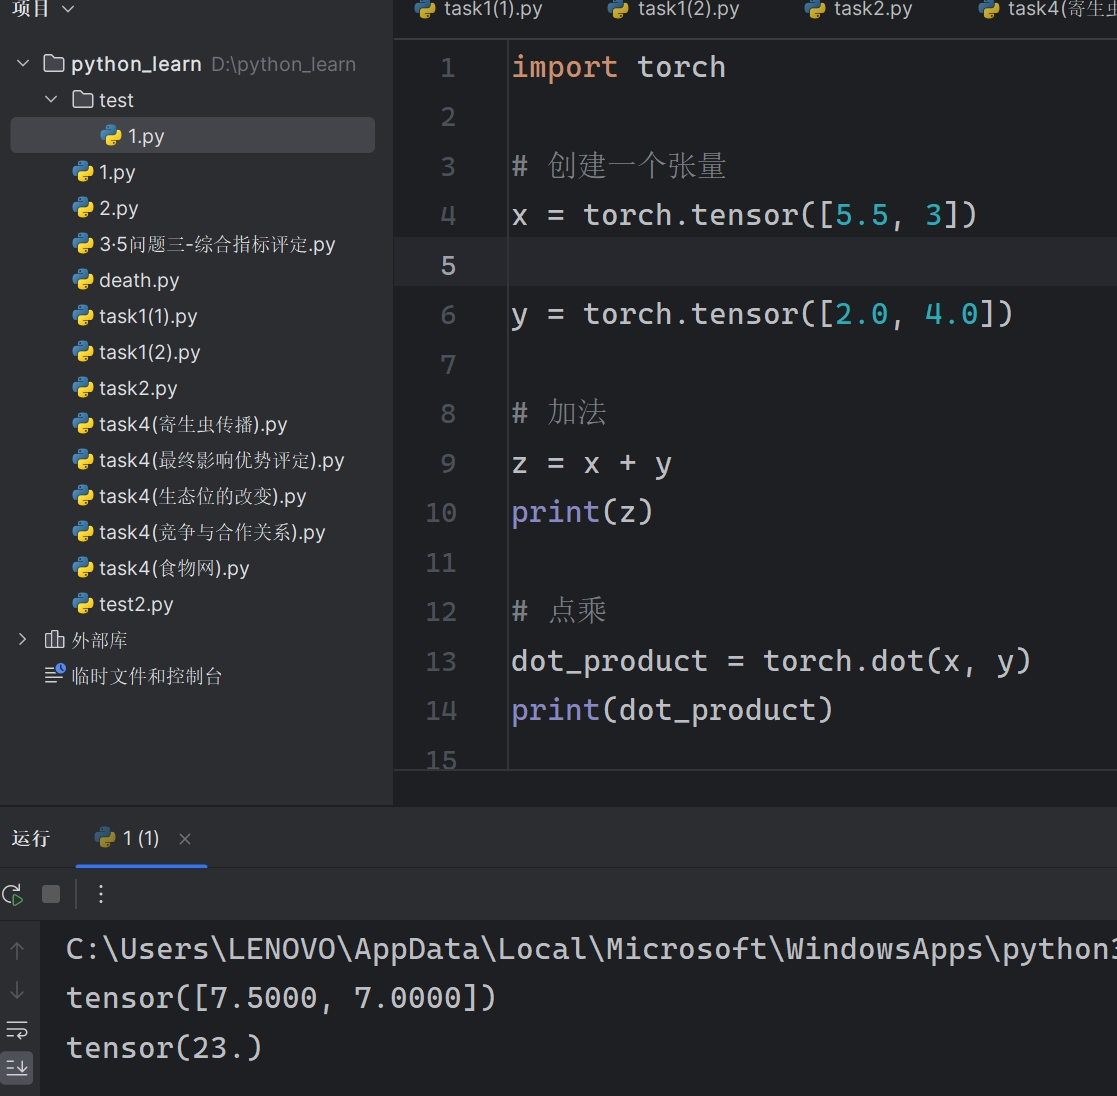
\includegraphics[width = 16cm]{45}
	
	\subsection{线性模型}
	通过在pycharm中导入pytorch库,来训练一个简单的线性模型,程序如下:
	
	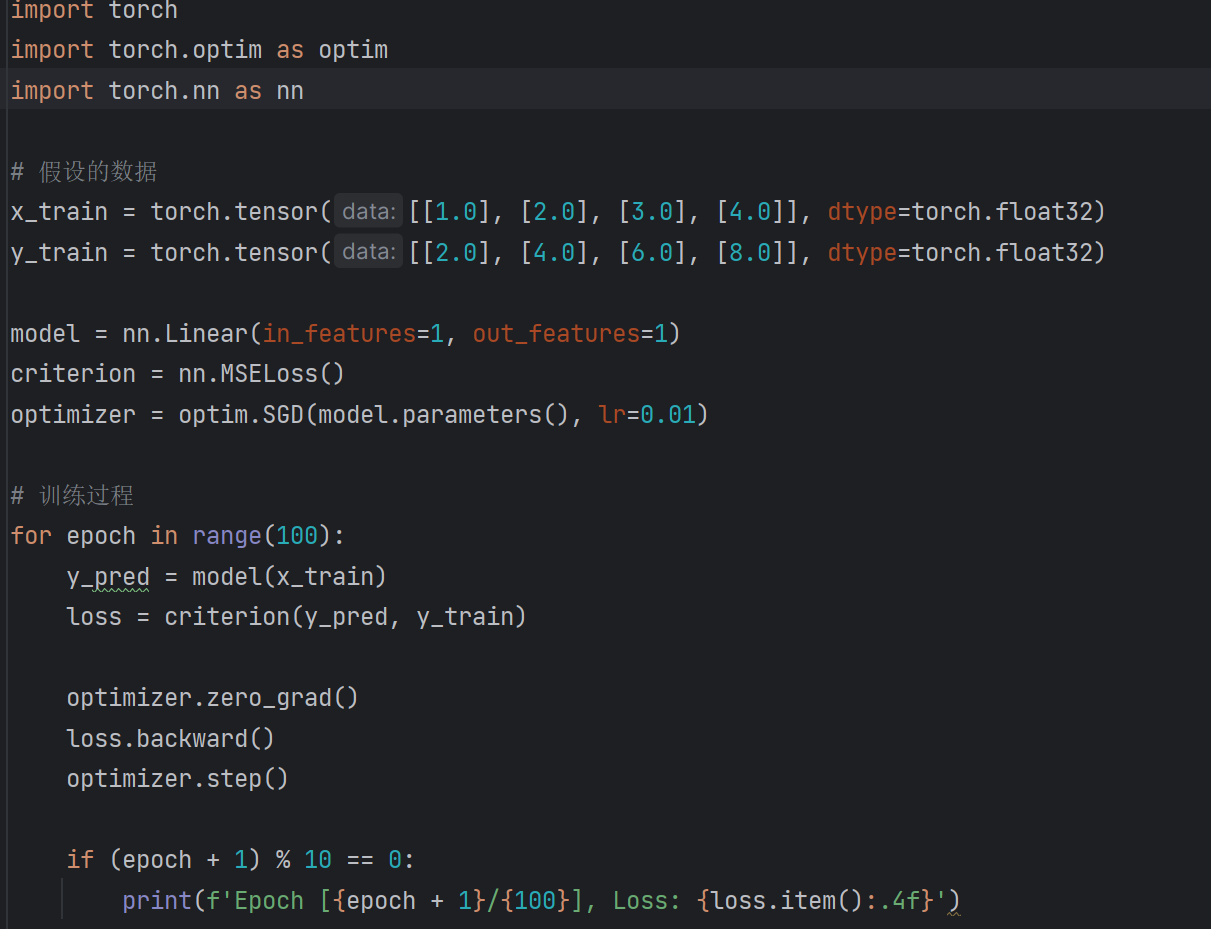
\includegraphics[width = 14cm]{39}
	
	运行结果为:
	
	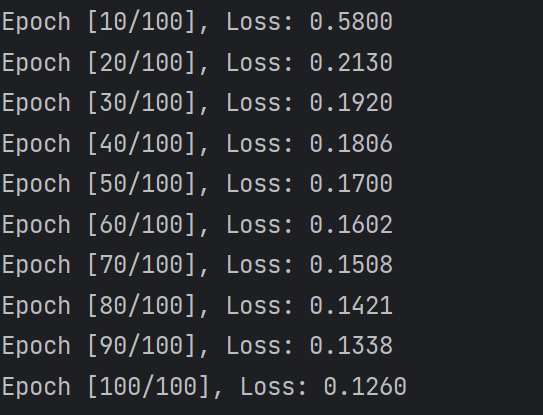
\includegraphics[width = 14cm]{40}
	
	
	\subsection{简单的全连接神经网络}
	简单的全连接网络是一种基本的神经网络结构,其中每一层的每个神经元都与上一层的所有神经元相连,以及与下一层的所有神经元相连。这种网络不包含卷积层或循环层,因此它没有空间或时间上的局部性概念,在此实例中,我参考教程后写出了一个简单的全连接神经网络,代买如下:
	
	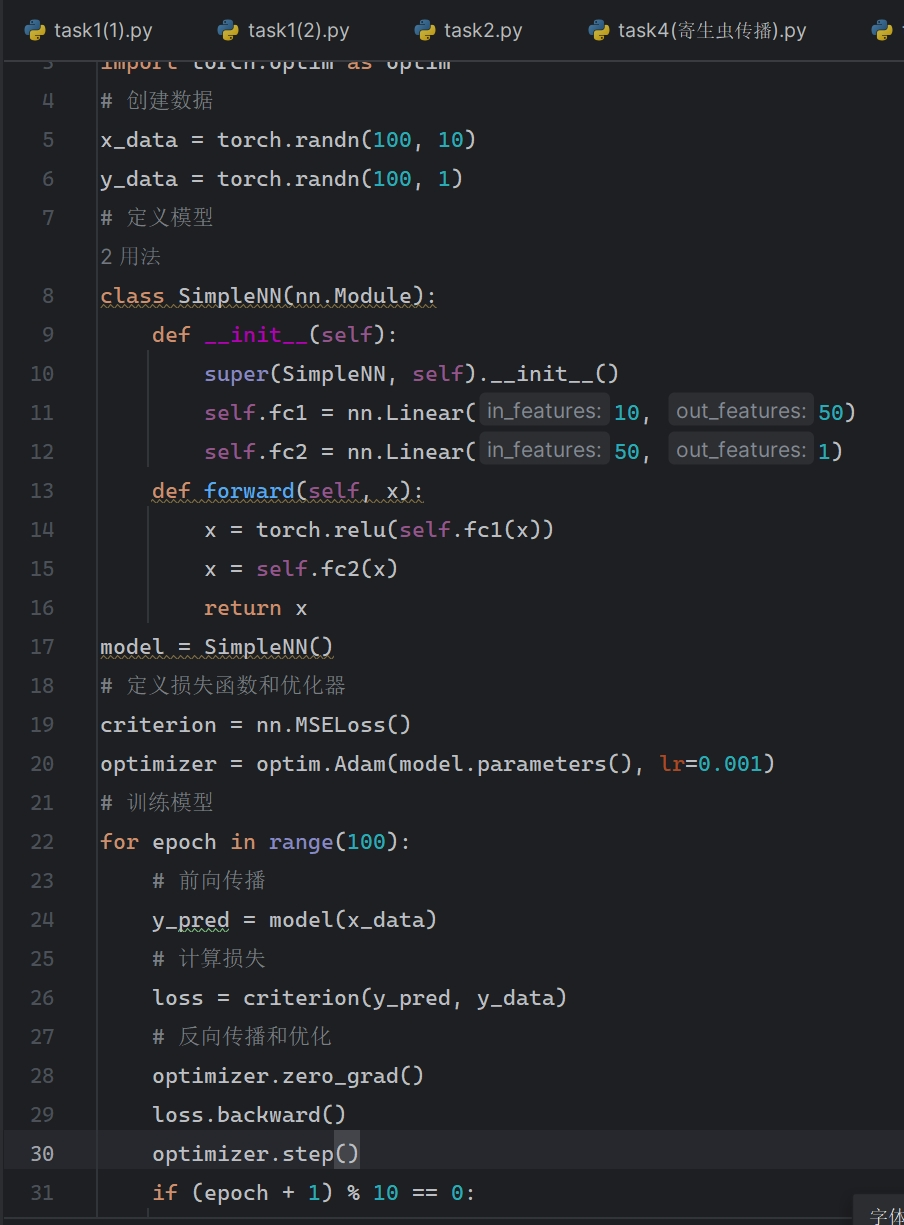
\includegraphics[width = 14cm]{41}
	
	在每个epoch结束时,代码将打印出当前epoch的编号和在该epoch结束时计算的损失值。
	
	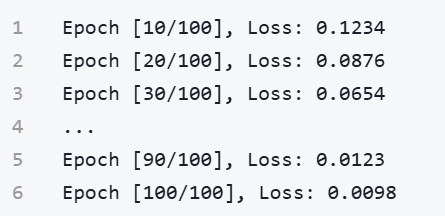
\includegraphics[width = 12cm]{42}
	
	\subsection{自动微分}
	在PyTorch中,自动微分是通过计算图来自动管理的,电脑根据自动微分向前和向后传播的差距来计算梯度。程序与运行结果如下:
	
	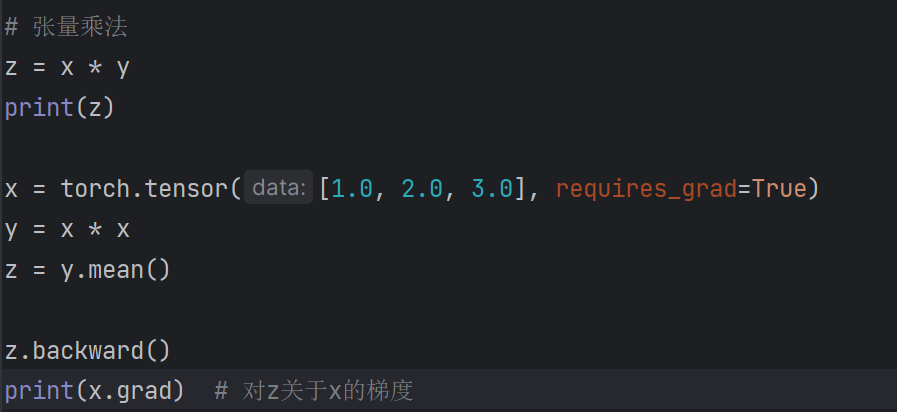
\includegraphics[width = 14cm]{43}
	
	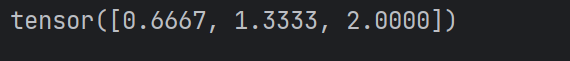
\includegraphics[width = 14cm]{44}
	
	\section{实验收获与感悟}
	在学习PyTorch的过程中,我深刻体会到代码调试与性能分析的重要性。PyTorch提供了丰富的调试和性能分析工具,如`print`语句、`set\_printoptions`和`profile`模块,它们帮助我更好地理解代码的执行流程和性能瓶颈。
	
	此外,我学会了使用GitHub进行版本控制和协作开发。GitHub是一个强大的平台,提供了分支管理、合并请求、代码审查等功能,使我能够更高效地管理和协作项目。
	
	在Markdown的学习过程中,我掌握了这种轻量级的标记语言,它可以让我更轻松地编写文档、笔记和博客。Markdown语法简单易懂,使我能够更高效地记录和分享知识。
	
	最后,我深入了解了PyTorch这个强大的深度学习框架。通过学习其最佳实践,如使用`torch.nn.Module`定义模型,使用`torch.optim`进行优化,使用`torchvision`进行数据预处理等,我能够更高效地开发和训练深度学习模型。
	
	总的来说,通过不断学习和实践,我提高了自己的技能和水平,也意识到了持续学习和实践的重要性。
	
	Github仓库链接:https://github.com/Locusclaer/-.git
	
\end{sloppypar}
\end{document}